\subsection{Steuerung}

Konnte einfache Kreise am Platz machen, gibt immer eine Abweichung mit der Ellipse und Geradeausfahrt\\

Der Roboter muss jetzt mit einer bestimmten Geschwindigkeit \(v\) und Winkelgeschwindigkeit \(\omega\) fahren. Zuerst muss die Kinematik des Roboters berechnet werden. Gegeben ist die kinematischen Matrix, die die Geschwindigkeiten der R"adern \(v_l, v_r\) zu der Geschwindigkeit des Achsmittelpunktes \(v_m\) und der Winkelgeschwindigkeit \(\omega\) verbinden,
\begin{equation}
    \begin{pmatrix}
        v_m \\
        \omega
    \end{pmatrix}
    =
    \begin{pmatrix}
        \nicefrac{1}{2} & \nicefrac{1}{2} \\
        \nicefrac{1}{-d} & \nicefrac{1}{d}
    \end{pmatrix}
    \begin{pmatrix}
        v_l \\
        v_r
    \end{pmatrix}
\end{equation}
mit \(d\) als die Achsenl"ange. 
Davon ist die inverse Matrix berechnet, sodass \(v_l\) und \(v_r\) von \(v_m\) und \(\omega\) ausgerechnet werden k"onnen:
\begin{equation}
    \begin{pmatrix}
        v_l \\
        v_r
    \end{pmatrix}
    = 
    \begin{pmatrix}
        1 & \nicefrac{-d}{2} \\
        1 & \nicefrac{d}{2}
    \end{pmatrix}
    \begin{pmatrix}
        v_m \\
        \omega
    \end{pmatrix}
    .
\end{equation} \\

Als n"achstes muss die Drehzahl den beiden R"adern berechnet werden. Das ist erfolgreich durch die folgende Gleichung:
\begin{equation}
    \omega_{l,r} = \dfrac{v_{l,r}}{R_{l,r}},
\end{equation}
mit \(R_{l,r}\) als die Radien der linken und rechten R"adern. \\

Letzlich muss die PWM-Werte \(u_{PWM,l,r}\) der Motoren berechnet werden. Obwohl der Zussamenhang zwischen die Drehzahlen \(\omega_{l,r}\) und die PWM-Werte nicht linear ist, d"urfte der Roboter dieser Zusammenhang als eine lineare Gleichung im Form von
\begin{equation}
    u_{PWM,l,r} = k_{m,l,r} \, \omega_{l,r} + u_{PWM,Y-Schnittpunkt,l,r}
\end{equation}
approximieren, weil der PWM-Wert von dem Y-Schnittpunkt linear steigt. \\

Die Motorenkonstanten \(k_{m,l,r}\) und PWM-Y-Schnittpunkten \(u_{PWM,Y-Schnittpunkt,l,r}\) werden experimentell bestimmt. Ein Program l"auft auf dem Roboter, das die PWM-Werte der Motoren von \si{0\percent} bis \si{100\percent} mit einer Rate von \si{1 \volt_{PWM}\per\second} hochfährt. Jede Sekunde werden die PWM-Werte und Drehzahlen der Motoren aufgenommen. Die aufgenommenen Werte werden in einer Tabelle geschrieben und einem Diagramm dargestellt. Die Drehzahlen sind auf dem X-Achse und die PWM-Werte sind auf dem Y-Achse. Durch lineare Regression wird zwei lineare Funktionen zwischen den Drehzahlen und den PWM-Werten bestimmt. Davon sind die Steigungen der Funktionen die Motorenkonstanten und Y-Schnittpunkte sind die PWM-Y-Werte. Mit dieser Funktion ist die Kette von \(v_m\) und \(\omega\) zu \(u_{PWM,l,r}\) fertig. \\

Mit dieser Methode kann der Roboter einfache Kreise am Platz fahren, aber der Roboter kann nicht ohne Abweichungen gerade  ausfahren und Ellipse fahren. Das liegt darauf, dass diese Methode nur eine Steuerung ist und nicht eine Regelung. Bei Steuerung hat die Ausgabe keinen Einfluss auf der Eingabe. Deshalb hat der Regelkreis einer Steuerung keine Gegenkopplung von Ausgabe zu Eingabe. Der Regelkreis der \(v/\omega\)-Steuerung ist in Abbildung \ref{fig:steuerung} zu sehen. Ohne dieser R"uckf"uhrung kann der Roboter nicht wissen wie schnell der f"ahrt. \\

\begin{figure}
    \centering
    \documentclass{standalone}
\usepackage{babel}
\usepackage{german}
\usepackage{textcomp}
\usepackage{tikz}
\usepackage{mathtools}
\usepackage{nicefrac}
\usetikzlibrary{shapes,arrows,positioning}
\begin{document}
\tikzset{
block/.style    = {draw, thick, rectangle, minimum height = 3em,
  minimum width = 3em},
sum/.style      = {draw, circle, node distance = 2cm, inner sep = 0pt,
minimum size = 0.5cm}, % Adder
input/.style    = {coordinate}, % Input
output/.style   = {coordinate} % Output
}
\newcommand{\suma}{\Large$+$}
\newcommand{\inte}{$\displaystyle \int$}
\newcommand{\derv}{\huge$\frac{d}{dt}$}
\begin{tikzpicture}[auto, thick, node distance=2cm, >=triangle 45]
\node [block] (matrix) {\(
        \begin{psmallmatrix}
            1 & \nicefrac{-d}{2} \\
            1 & \nicefrac{d}{2} 
        \end{psmallmatrix}
    \)}
;
\node [input, left=of matrix.160] (vm) {};
\node [input, left=of matrix.200] (w) {};

\node [block, right=of matrix] (radius) {\(\dfrac{1}{R_{l,r}}\)};
\node [input, right=of matrix.20] (vl) {\(v\)};
\node [input, right=of matrix.340] (vr) {\(\omega\)};

\node [block, right=of radius] (function) {Steuerung};
\node [input, right=of radius.30] (wl) {};
\node [input, right=of radius.330] (wr) {};

\node [input, right=of function.20] (ul) {};
\node [input, right=of function.340] (ur) {};

\draw[->] (vm) -- node {\(v_m\)} (matrix.160);
\draw[->] (w) -- node [below] {\(\omega\)} (matrix.200);

\draw[->] (matrix.20) -- node {\(v_l\)} (vl);
\draw[->] (matrix.340) -- node [below] {\(v_r\)} (vr);

\draw[->] (radius.30) -- node {\(\omega_l\)} (wl);
\draw[->] (radius.330) -- node [below] {\(\omega_r\)} (wr);

\draw[->] (function.20) -- node {\(u_{PWM,l}\)} (ul);
\draw[->] (function.340) -- node [below] {\(u_{PWM,r}\)} (ur);

\end{tikzpicture}
\end{document}
    \caption{\(v/\omega\)-Steuerung}
    \label{fig:steuerung}
\end{figure}


\subsection{Regelung}

Bei der Einführung eines Reglers ist das Verhalten des \(v/\omega\)-Steuerung viel genauerer. Der Regelkreis mit dem Regler ist in Abbildung 3 zu sehen. Aber am Anfang lief der Roboter nicht problemlos. Mit der ersten Version des Reglers fährt der Roboter ziemlich genau gerade mit einer pr"azisen Geschwindigkeit, aber der Roboter konnte nicht am Platz mit einer präzisen Drehgeschwindigkeit drehen. Der Roboter w"urde immer ein bisschen zu wenig drehen. Diese Problem lag an der Nichtlinearität des Motors. Jeder Motor hat eine bestimmte tote Zone oder in englischen “Deadzone”, die der Motor beseitigen muss, bevor er anfangen kann, zu drehen. Die tote Zone kommt von der inneren Reibung des Motors und muss bei jedem Regler berücksichtigt werden. \\

Eine Methode, um diese tote Zone zu kompensieren, ist durch die Implementation einer Steuerung. Weil der Roboter schon eine Steuerung hatte, konnte der Roboter gerade fahren. Aber mit nur dieser Steuerung konnte der Roboter problemlos drehen. Deswegen wird ein Arbeitspunkt zu dem Regler hinzufügt. \\

Die zweite Version des Reglers hat ein richtig präzise Führungsverhalten mit dem gerade Fahren und Drehen. Aber der Arbeitspunkt des Reglers liefert eine ziemlich hohe "Uberschwingung zu der Regelstrecke, die manchmal zwingt, der Roboter zu weit zu drehen. Die "Uberschwingung ist in Abbildung \ref{fig:vw-control} zu sehen. \\ 

\begin{figure}
    \centering
    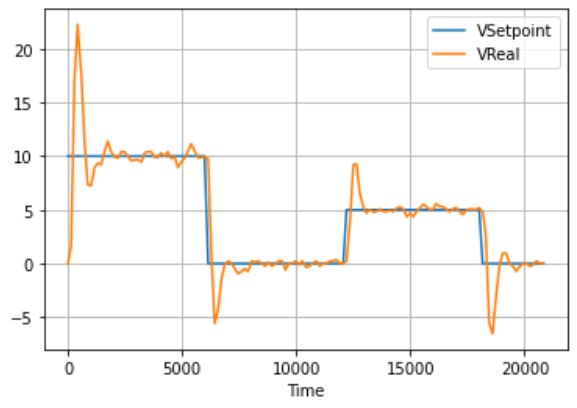
\includegraphics{vw-control}
    \caption{"Uberschwingung}
    \label{fig:vw-control}
\end{figure}

Die dritte Version des Reglers implementiert eine nichtlineare Funktion, um den Arbeitspunkt des Regler zu setzen. Bei niedriger Geschwindigkeit und Drehgeschwindigkeit wird der Arbeitspunkt hoch gesetzt, um die tote Zone zu kompensieren, und bei hoher Geschwindigkeit und Drehgeschwindigkeit wird er tiefer gesetzt. Die nichtlineare Funktion wird benötigt, weil der Arbeitspunkt plus Steuerung zusammen eine Überkompensation zu der Regelstrecke liefert. Deswegen wird der Arbeitspunkt tiefer, wenn er bei hoher Geschwindigkeit und Drehgeschwindigkeit nicht mehr benötigt ist. Der fertige Regelkreis ist in Abbildung \ref{fig:regelung} zu sehen. \\

\begin{figure}
    \centering
    % Title: Block diagram of Third order noise shaper in Compact Disc Players
% Author: Ramón Jaramillo
\documentclass{standalone}
\usepackage{babel}
\usepackage{german}
\usepackage{textcomp}
\usepackage{tikz}
\usetikzlibrary{shapes,arrows}
\begin{document}
% Definition of blocks:
\tikzset{
block/.style    = {draw, thick, rectangle, minimum height = 3em,
  minimum width = 3em},
sum/.style      = {draw, circle, node distance = 2cm, inner sep = 0pt,
minimum size = 0.5cm}, % Adder
input/.style    = {coordinate}, % Input
output/.style   = {coordinate} % Output
}
% Defining string as labels of certain blocks.
\newcommand{\suma}{\Large$+$}
\newcommand{\inte}{$\displaystyle \int$}
\newcommand{\derv}{\huge$\frac{d}{dt}$}
\begin{tikzpicture}[auto, thick, node distance=2.25cm, >=triangle 45]
\draw
% Drawing the blocks of first filter :
    node at (0,0) [right=0mm]{}
    node [input] (input1) {} 
    node [right of=input1] (branch1) {}
    node [sum, right of=branch1] (suma1) {\suma}
    node [block, above of=suma1] (steuerung) {Steuerung}
    node [block, right of=suma1] (PID) {PID}
    node [sum, right of=PID] (suma2) {\suma}
    node [block, right of=suma2] (plant) {Regelstrecke}
    node [right of=plant] (branch2) {}
    node [block, below of=suma2] (branch3) {Encoder}
;

% Joining blocks. 
% Commands \draw with options like [->] must be written individually
\draw[-] (input1) -- node {\(\omega_{l,r}\)} (branch1.center);
\draw[->] (branch1.center) -- (suma1);
\draw[-] (branch1.center) |- (steuerung);
\draw[->] (steuerung) -| (suma2);
\draw[-] (suma1) -- (PID);
\draw[->] (PID) -- (suma2);
\draw[-] (suma2) -- (plant);
\draw[-] (plant) -- (branch2.center);
\draw[-] (branch2.center) |- (branch3);
\draw[->] (branch3) -| node[pos=0.30, label={\(\omega_{Real,l,r}\)}] {} node[pos=0.97, xshift=-5] {\huge $-$} (suma1);

\filldraw
  (branch1) circle (2pt)
;
\end{tikzpicture}
\end{document}
    \caption{\(v/\omega\)-Regelung}
    \label{fig:regelung}
\end{figure}

Die Implementierung der dritten Version des Reglers auf dem Roboter erlaubt die pr"asizen Bewegungen von Kreisen und Ellipsen. Der Roboter kann auch f"ur ziemlich weite Strecken auch gerade fahren. Manchmal dreht er sich ein bisschen zu weit, aber das ist selten.

